

\documentclass[../../main.tex]{subfiles}


\begin{document}
\section{OpAmp}
\subsection{Introducci\'on}
Se analizaron dos circuitos con Amplificadores operacionales. El primero es un circuito inversor, cuya salida es opuesta a la entrada y  la aplifica o atenua, de a cuerdo a como se configure. El segundo es no inversor, igual que el primero, atenua o amplifica la señal de entrada, pero no la invierte.
El objetivo es evaluar las caracteristicas lineales y no lineales de los amplificadores operacionales. Tambien la respuesta en frecuencia y la respuesta  distintos valores de tensiones de entrada.


\subsection{Circuito inversor}
\todo{algo desir alog}


\begin{figure}[H]
\centering

\begin{circuitikz}[scale=1]
\def\xspacing{2}
\def\xstart{0}
\def\yspacing{2}	
\def\ystart{0}

%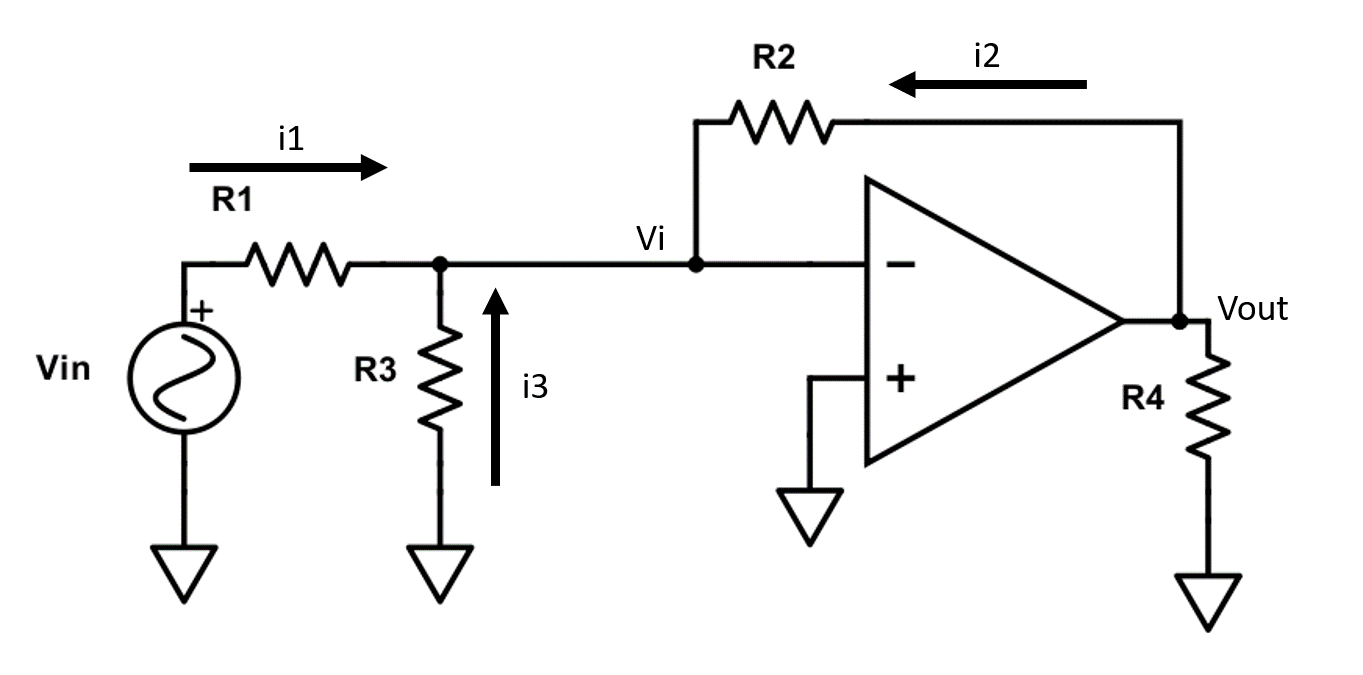
\includegraphics[width=0.5\textwidth]{imagenes/xxx.png}




%dibujo malla izquierda
\draw   						(\xstart, \ystart) node[ground]{}
		to [vsourcesin]	 	(\xstart, \ystart + \yspacing)
		to [R=$R_1$, i>^=$i_1$] (\xstart + \xspacing, \ystart + \yspacing)
		to [R=$R_3$, i<^=$i_3$] (\xstart + \xspacing, \ystart)
		to (\xstart + \xspacing, \ystart) node[ground]{}

%dibujo opamp
%el opamp tiene la misma altura que scale, y las patitas - y + estan en .25*scale y .75*scale
%nos queda - en ystart+yspacing y + en ystart+spacing-0.5

		(\xstart + 3*\xspacing, \ystart + \yspacing - .5) node[op amp] (opamp) {}

%dibujo conexiones a opamp
	 						   (\xstart + \xspacing, \ystart + \yspacing)
		to [short]			  (opamp.-)
								(opamp.+)
		to [short]			  ($(opamp.+)+(0,-\yspacing + 1)$) node[ground]{}	%se me va la patita
								(\xstart + 2*\xspacing, \ystart + 1*\yspacing)
		to [short, *-]		  (\xstart + 2*\xspacing, \ystart + 1.7*\yspacing)
		to [R=$R_2$, i<^=$i_2$] (\xstart + 4*\xspacing, \ystart + 1.7*\yspacing)
		to [short, -*]		  (\xstart + 4*\xspacing, \ystart + 1*\yspacing -.5)
		to [short]			  (opamp.out)
								(\xstart + 4*\xspacing, \ystart + 1*\yspacing -.5)
		to [R=$R_4$]			(\xstart + 4*\xspacing, \ystart) node[ground]{};


\end{circuitikz}


\caption{Esquematico del circuito Inversor}
\end{figure}

Los valores de las resistencias utilizados fueron los indicados en la Tabla \ref{tab=vResistencias}.

\begin{table}[h]
\begin{center}
\begin{tabular}{|l|l|l|l|}
\hline
Caso & $R_{1}=R_{3}$ & $R_{2}$ & $R_{4}$\\
\hline \hline
1 & $5 K\Omega $ &  $50 K\Omega $ &  $20 K\Omega $ \\ \hline
2 & $5 K\Omega $ &  $5 K\Omega $ &  $20 K\Omega $ \\ \hline
3 & $50 K\Omega $ &  $5 K\Omega $ &  $100 K\Omega $ \\ \hline
\end{tabular}
\caption{Valores de resistensias.} 
\label{tab=vResistencias}
\end{center}
\end{table}



\subsubsection{Caso $A_{vol}$ infinito}

Como $A_{vol}$ lo consideramos infinito, $V_{i}=0$ \big( tierra virtual \big).Por ende $i_{3}=0$ e $i_{2}=-i_{1}$, Ademas no circula corriente por la entrada del   amplificador operacional.
\begin{gather}
V_{out}=-\frac{i_{1}}{R_{2}}\label{eq=CircuitoA6}\\
i_{1}=\frac{V_{in}}{R_{1}}\label{eq=CircuitoA7}
\end{gather}
Reemplazando \ref{eq=CircuitoA7} en \ref{eq=CircuitoA6} y operando algebraicamente se obtine:
\begin{equation}
\frac{V_{out}}{V_{in}}= -\frac{R_{2}}{R_{1}} \label{eq=CircuitoAideal}
\end{equation}


\subsubsection{Caso $A_{vol}$ finito}

Como $A_{vol}$  lo consideramos finito, $V^{+}\neq V^{-}$ . Se considera que no circula corriente por  los terminales de entrada del amplificador operacional, devido a la alta impedancia que hay entre ellos.

\begin{gather}
V_{out}= -V_{i}\cdot A_{vol}\label{eq=CircuitoA1}\\
i_{1}=\frac{V_{in}-V{i}}{R_{1}}\label{eq=CircuitoA2}\\
i_{2}=\frac{V_{out}-V_{i}}{R_{2}}\label{eq=CircuitoA3}\\
i_{3}=\frac{-V_{i}}{R_{3}}\label{eq=CircuitoA4}\\
i_{1}+i_{2}+i_{3}=0\label{eq=CircuitoA5}
\end{gather}

Reemplazando \ref{eq=CircuitoA1},\ref{eq=CircuitoA2},\ref{eq=CircuitoA3},\ref{eq=CircuitoA4} en \ref{eq=CircuitoA5}, se obtiene:


$$\frac{V_{in}}{R_{1}} + \frac{V_{out}}{R_{2}}+\frac{V_{out}}{A_{vol}}\cdot \bigg( \frac{1}{R_{1}} + \frac{1}{R_{2}} + \frac{1}{R_{3}} \bigg) = 0$$

Operando algebraicamente, se obtiene:

\begin{equation}
\frac{V_{out}}{V_{in}}= - \frac{A_{vol} \cdot R_{2} \cdot R_{3}}{A_{vol}\cdot R_{1} \cdot R_{3} + R_{2} \cdot R_{3} +  R_{1} \cdot R_{3} + R_{1} \cdot R_{2} }\label{eq=gananciaAfinito}
\end{equation}
Observacion

$$ \lim_{A_{vol}\to\infty} \big( \ref{eq=gananciaAfinito} \big) = -\frac{R_{2}}{R_{1}} $$
La expresion se redujo a la ganancia del circuito, con el apmlificador operacional ideal\\ \big(\ref{eq=CircuitoAideal}\big).

\subsubsection{Caso $A_{vol}$  con polo dominante}

\begin{equation}
A_{vol }=\frac{A_{0}}{1+\frac{s}{W_{p}}}\label{eq=AvolWp}\\
\end{equation} 

Reemplazando \big(\ref{eq=AvolWp}\big) en  \big(\ref{eq=gananciaAfinito}\big)  se obtiene:

\begin{equation}
\frac{V_{out}}{V_{in}}= - \frac{\frac{A_{0}}{1+\frac{s}{W_{p}}} \cdot R_{2} \cdot R_{3}}{\frac{A_{0}}{1+\frac{s}{W_{p}}}\cdot R_{1} \cdot R_{3} + R_{2} \cdot R_{3} +  R_{1} \cdot R_{3} + R_{1} \cdot R_{2} }
\end{equation}

Llamando $K= R_{2} \cdot R_{3} +  R_{1} \cdot R_{3} + R_{1} \cdot R_{2}$


\begin{equation}
\frac{V_{out}}{V_{in}}=- \frac{A_{0} \cdot  R_{2} \cdot  R_{3} }{A_{0} \cdot R_{1} \cdot  R_{3} + K }  \cdot \frac{1}{1 +\frac {S}{\frac{W_{p}  \cdot \big( A_{0} \cdot R_{1} \cdot R_{3} + K \big) }{K}}} \label{eq=poloDominante}
\end{equation}

 Despejando se obtiene la frecuencia de corte del circuito:
\begin{equation}
f_{P}=\left( \frac {A_{0} \cdot R_{1} \cdot R_{3} + K}{K}\right)  \cdot \frac{W_{P}}{2\cdot \pi}  \label{eq=fCorte}
\end{equation}

\textit{Observacion:}  la ecuacion \big(\ref{eq=poloDominante} \big) posee la misma forma que la funcion transferencia de un pasabajos.



El amplificador operacional utilizado fue el LM324 de ON Semiconductor, de la hoja de datos se obtuvieron las siguientes cararacteristicas del integrado:


\begin{table}[h]
\begin{center}
\begin{tabular}{|l|l|}
\hline
$A_{0}$ & $f_{P}$ \\
\hline \hline
$10\cdot 10^{4}$& $ 12Hz $ \\ \hline

\end{tabular}
\caption{Caracteristicas del LM324} 
\label{tab=lm324Carac}
\end{center}
\end{table}
Donde $A_{0}$ es la ganancia del amplificador operacional a lazo abierto y  $f_{P}$ es la frecuencia de corte a lazo abierto. A partir de las tablas \ref{tab=vResistencias} y \ref{tab=lm324Carac} y de ecuación  \ref{eq=poloDominante}, se calcularon las caracteristicas de las tres configuraciones del circuito analizadas.

\begin{table}[h]
\begin{center}
\begin{tabular}{|l|l|l|l|}
\hline
Caso &Ganancia ideal & Ganancia $A_{vol}$ finito & Frecuencia de corte\\
\hline \hline
1 & $-10$ & -9,997 & 54,7$KHz$ \\ \hline
2 & $-1$ &  $-0,999 $ &  386$KHz$  \\ \hline
3 & $-0,1$ &- 0,099 &960$KHz$\\ \hline
\end{tabular}
\caption{Ganancia y frecuencia de corte del circuito.La ganancias es en veces.} 
\label{tab=gananciayFrecCorte}
\end{center}
\end{table}

Acontinuacion se graficaran los tres casos del circuito inversor, comparando $A_{vol}$ infinito y $A_{vol}$ con polo dominante.


\subsection{Circuito no inversor}


\end{document}
